\chapter{Generación de relojes}
\label{cha:mmcm}

En relación a la generación de señales de reloj, se ha decidido implementar un bloque MMCM en el último proyecto de Vivado, perteneciente al bloque del mezclador (ver Capítulo \ref{section:mezcla}).

%FIGURA ESQUEMA

\vspace{3mm}

El objetivo es hacer un uso práctico de este bloque en uno de los módulos del sistema para validar su funcionamiento, mientras que en el resto se trasladaría directamente la señal de reloj correspondiente. Se considera partir de un reloj externo de frecuencia igual a 36 MHz para generar a la salida tres relojes: de 576 MHz (DDS/Multiplicadores), 192 MHz (RRC)
y 52 MHz (XADC). 

\vspace{3mm}

Para ello, se añaden al proyecto dos bloques IP: \textit{Simulation Clock Generation}, para generar el reloj externo y \textit{Clocking Wizard}, para obtener las tres salidas de reloj con diferentes frecuencias. En la Figura \ref{fig:mmcm} se puede observar la configuración del bloque IP para la generación de relojes \textit{Clocking Wizard}.

\vspace{3mm}

\begin{figure}[h]
	\centering
	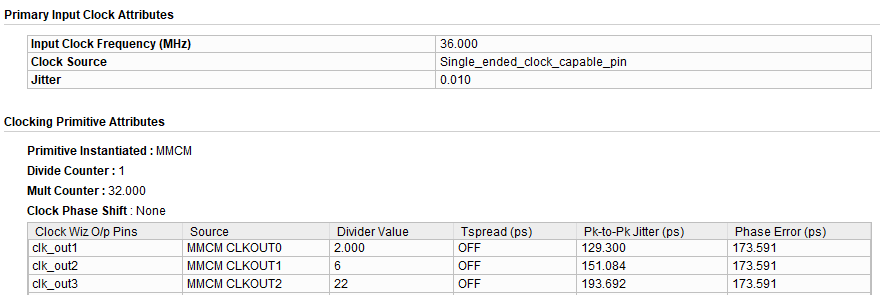
\includegraphics[width=1\textwidth, height=6cm]{img/diseno/mmcm.PNG}
	\caption{Resumen de configuración del bloque IP \textit{Clocking Wizard}}
	\label{fig:mmcm}
\end{figure}

\pagebreak

Como se implementa en el módulo del mezclador, se cogerá la salida con frecuencia 576 MHz y se conectará la misma a todos los bloques.

\vspace{3mm}

\begin{figure}[h]
	\centering
	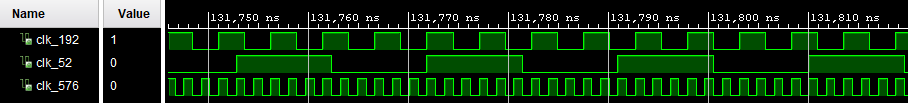
\includegraphics[width=1\textwidth, height=2.5cm]{img/simu/mmcm.PNG}
	\caption{Comprobación del funcionamiento del bloque IP \textit{Clocking Wizard}}
	\label{fig:mmcm2}
\end{figure}



